\documentclass[aspectratio=169, 10pt]{beamer}
\usetheme{metropolis}
% \usefonttheme{professionalfonts}

\usepackage[english]{babel}
\usepackage[style=authortitle,backend=biber]{biblatex}
\usepackage[utf8]{inputenc}
\usepackage{algorithmic}
\usepackage{amsfonts}
\usepackage{amsmath}
\usepackage{amssymb}
\usepackage{array}
\usepackage{booktabs}
\usepackage{caption}
\usepackage{colortbl}
\usepackage{csquotes}
\usepackage{graphicx}
\usepackage{heuristica}
\usepackage{hyperref}
\usepackage{mathptmx}
\usepackage{multirow}
\usepackage{pgfplots}
\usepackage{siunitx}
\usepackage{subcaption}
\usepackage{svg}
\usepackage{tabularx}
\usepackage{textcomp}
\usepackage{xcolor}

\addbibresource{references.bib}

\usetikzlibrary{calc}

% \pgfplotsset{compat=1.17}
\usepgfplotslibrary{statistics}

\definecolor{uniblue}{HTML}{00467f}
\definecolor{uniblueDark}{HTML}{002052}
\definecolor{uniblueLight}{HTML}{4671af}
\definecolor{blueGrey}{HTML}{cfd8dc}
\definecolor{red800Dark}{HTML}{8e0000}
\definecolor{green800Dark}{HTML}{005005}

\setbeamercolor{background canvas}{bg=white}
% \setbeamertemplate{frame footer}{\insertshortauthor}
\setbeamerfont{page number in head/foot}{size=\tiny}
% \setbeamercolor{footline}{fg=white, bg=uniblue}
\setbeamercolor{footline}{fg=uniblue}
\setbeamercolor{title}{fg=uniblueDark, bg=white}
\setbeamercolor{frametitle}{fg=white, bg=uniblue}
\setbeamercolor{progress bar}{fg=uniblueLight, bg=white}
\setbeamercolor{block title}{use=structure,fg=white,bg=uniblue}
\setbeamercolor{block body}{use=structure,fg=black,bg=blueGrey}
\setbeamercolor{block title alerted}{fg=white,bg=red800Dark}
\setbeamercolor*{block title example}{fg=white, bg=green800Dark}
\setbeamercolor{alerted text}{fg=red800Dark}
\setbeamercolor{footnote}{fg=black}
\setbeamertemplate{frametitle continuation}[from second]
\setbeamercolor*{bibliography entry title}{fg=black}
\setbeamercolor*{bibliography entry author}{fg=black}
\setbeamercolor*{bibliography entry location}{fg=black}
\setbeamercolor*{bibliography entry note}{fg=black}
% \setbeamertemplate{bibliography item}{}

\setbeamerfont{author}{size=\normalsize}
\setbeamerfont{institute}{size=\small}
\setbeamerfont{date}{size=\normalsize}

\newcommand{\vect}{\mathbf}

\DeclareMathOperator*{\argmax}{argmax}

\hypersetup{
    colorlinks=false,
    linkcolor=blue,
    filecolor=blue,      
    urlcolor=blue,
}

\title{COMPSCI 762 Tutorial 8}
% \subtitle{Tutorial on Bayesian Networks, kNN, SVM, MDP and Q-Learning}
\subtitle{Tutorial on Bayesian Networks, kNN and SVM}
\author{Luke Chang}
\institute{The University of Auckland}
\date{May 2021}


\begin{document}

\frame{\titlepage}

% %-------------------------------------------------------------------------------
\begin{frame}
    \frametitle{Topics}

    \tableofcontents
        
\end{frame}

%-------------------------------------------------------------------------------
\section{Bayesian Networks}
\begin{frame}[t]
    \frametitle{Bayesian Networks}

    \begin{example}
        You are given a toxicity data set that describes chemical compounds with 5 \textit{Boolean}
        attributes: water \textbf{S}olubility, \textbf{C}ytochrominhibitor, contains \textbf{P}hosphate, and
        cancerogenic in the \textbf{R}at model, and the \textbf{O}utcome of some toxicity test.\\
        Could you learn a Bayesian network on the given dataset?
    \end{example}
    
    \begin{table}[]
        \small
        \begin{tabular}{cccc|c}
        \textbf{S} & \textbf{C} & \textbf{P} & \textbf{R} & \textbf{O} \\ \hline
        TRUE       & TRUE       & FALSE      & TRUE       & Negative   \\
        TRUE       & FALSE      & TRUE       & TRUE       & Negative   \\
        FALSE      & FALSE      & TRUE       & FALSE      & Negative   \\
        FALSE      & TRUE       & TRUE       & TRUE       & Positive  
        \end{tabular}
    \end{table}

    \vspace{2em}
    If you condition on every attribute (join links top down), \textbf{O} will condition on $4!=24$ possible combinations.
\end{frame}

%-------------------------------------------------------------------------------
\begin{frame}[t]
    \frametitle{Bayesian Networks}

    \begin{columns}[]
        \begin{column}[]{0.5\textwidth}
            \begin{table}[]
                \small
                \begin{tabular}{cccc|c}
                \textbf{S} & \textbf{C} & \textbf{P} & \textbf{R} & \textbf{O} \\ \hline
                TRUE       & TRUE       & FALSE      & TRUE       & Negative   \\
                TRUE       & FALSE      & TRUE       & TRUE       & Negative   \\
                FALSE      & FALSE      & TRUE       & FALSE      & Negative   \\
                FALSE      & TRUE       & TRUE       & TRUE       & Positive  
                \end{tabular}
            \end{table}
        \end{column}
        \begin{column}[]{0.5\textwidth}
            \begin{figure}
                \center
                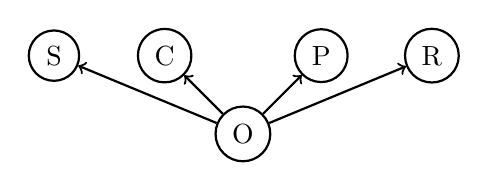
\begin{tikzpicture}[node distance={4em}, thick, main/.style = {draw, circle}] 
                    \node[main] (1) {O};
                    \node[main] (2) [above left of=1] {C};
                    \node[main] (3) [above right of=1] {P};
                    \node[main] (4) [left of=2] {S};
                    \node[main] (5) [right of=3] {R};
        
                    \draw[<-] (2) -- (1); 
                    \draw[<-] (3) -- (1); 
                    \draw[<-] (4) -- (1); 
                    \draw[<-] (5) -- (1); 
                \end{tikzpicture} 
            \end{figure}
        \end{column}
    \end{columns}

    \begin{table}[]
        \small
        \begin{tabular}{cc}
        P(O) & P($\neg$O) \\ \hline
        0.25 & 0.75 \\
        \end{tabular}
    \end{table}

    \begin{columns}
        \begin{column}{0.25\textwidth}
            \begin{table}[]
                \small
                \begin{tabular}{ccc}
                O & P(S) & P($\neg$S) \\ \hline
                P & \textcolor{red}{0.0} & 1.0 \\
                N & 0.666 & 0.333 \\
                \end{tabular}
            \end{table}
        \end{column}
        \begin{column}{0.25\textwidth}
            \begin{table}[]
                \small
                \begin{tabular}{ccc}
                O & P(C) & P($\neg$C) \\ \hline
                P & 1.0 & \textcolor{red}{0.0} \\
                N & 0.333 & 0.666 \\
                \end{tabular}
            \end{table}
        \end{column}
        \begin{column}{0.25\textwidth}
            \begin{table}[]
                \small
                \begin{tabular}{ccc}
                O & P(P) & P($\neg$P) \\ \hline
                P & 1.0 & \textcolor{red}{0.0} \\
                N & 0.666 & 0.333 \\
                \end{tabular}
            \end{table}
        \end{column}
        \begin{column}{0.25\textwidth}
            \begin{table}[]
                \small
                \begin{tabular}{ccc}
                O & P(R) & P($\neg$R) \\ \hline
                P & 1.0 & \textcolor{red}{0.0} \\
                N & 0.666 & 0.333 \\
                \end{tabular}
            \end{table}
        \end{column}
    \end{columns}

    Apply Laplace smoothing

\end{frame}

%-------------------------------------------------------------------------------
\begin{frame}[t]
    \frametitle{Laplace smoothing}

    \begin{columns}[]
        \begin{column}[]{0.5\textwidth}
            \begin{table}[]
                \small
                \begin{tabular}{cccc|c}
                \textbf{S} & \textbf{C} & \textbf{P} & \textbf{R} & \textbf{O} \\ \hline
                TRUE       & TRUE       & FALSE      & TRUE       & Negative   \\
                TRUE       & FALSE      & TRUE       & TRUE       & Negative   \\
                FALSE      & FALSE      & TRUE       & FALSE      & Negative   \\
                FALSE      & TRUE       & TRUE       & TRUE       & Positive  
                \end{tabular}
            \end{table}
        \end{column}
        \begin{column}[]{0.5\textwidth}
            \begin{table}[]
                \small
                \begin{tabular}{cc}
                P(O) & P($\neg$O) \\ \hline
                $\frac{1+1}{4+2}=0.333$ & $\frac{3+1}{4+2}=0.666$ \\
                \end{tabular}
            \end{table}
        \end{column}
    \end{columns}

    \begin{columns}
        \begin{column}{0.5\textwidth}
            \begin{table}[]
                \small
                \begin{tabular}{lll}
                O & P(S) & P($\neg$S) \\ \hline
                P & $\frac{0+1}{1+2}=0.333$ & $\frac{1+1}{1+2}=0.666$ \\
                N & $\frac{2+1}{3+2}=0.6$ & $\frac{1+1}{3+2}=0.4$ \\
                \end{tabular}
            \end{table}

            \begin{table}[]
                \small
                \begin{tabular}{lll}
                O & P(C) & P($\neg$C) \\ \hline
                P & $\frac{1+1}{1+2}=0.666$ & $\frac{0+1}{1+2}=0.333$ \\
                N & $\frac{1+1}{3+2}=0.4$ & $\frac{2+1}{3+2}=0.6$ \\
                \end{tabular}
            \end{table}
        \end{column}
        \begin{column}{0.5\textwidth}
            \begin{table}[]
                \small
                \begin{tabular}{lll}
                O & P(P) & P($\neg$P) \\ \hline
                P & $\frac{1+1}{1+2}=0.666$ & $\frac{0+1}{1+2}=0.333$ \\
                N & $\frac{2+1}{3+2}=0.6$ & $\frac{1+1}{3+2}=0.4$ \\
                \end{tabular}
            \end{table}

            \begin{table}[]
                \small
                \begin{tabular}{lll}
                O & P(R) & P($\neg$R) \\ \hline
                P & $\frac{1+1}{1+2}=0.666$ & $\frac{0+1}{1+2}=0.333$ \\
                N & $\frac{2+1}{3+2}=0.6$ & $\frac{1+1}{3+2}=0.4$ \\
                \end{tabular}
            \end{table}
        \end{column}
    \end{columns}

\end{frame}

%-------------------------------------------------------------------------------
\begin{frame}[t]
    \frametitle{Bayesian Networks}

    \begin{figure}
        \center
        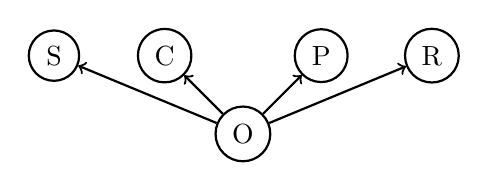
\begin{tikzpicture}[node distance={4em}, thick, main/.style = {draw, circle}] 
            \node[main] (1) {O};
            \node[main] (2) [above left of=1] {C};
            \node[main] (3) [above right of=1] {P};
            \node[main] (4) [left of=2] {S};
            \node[main] (5) [right of=3] {R};

            \draw[<-] (2) -- (1); 
            \draw[<-] (3) -- (1); 
            \draw[<-] (4) -- (1); 
            \draw[<-] (5) -- (1); 
        \end{tikzpicture} 
    \end{figure}

    \begin{table}[]
        \small
        \begin{tabular}{cc}
        P(O) & P($\neg$O) \\ \hline
        \textcolor{red}{0.333} & 0.666 \\
        \end{tabular}
    \end{table}

    \begin{columns}
        \begin{column}{0.25\textwidth}
            \begin{table}[]
                \small
                \begin{tabular}{ccc}
                O & P(S) & P($\neg$S) \\ \hline
                P & \textcolor{red}{0.333} & 0.666 \\
                N & 0.6 & 0.4 \\
                \end{tabular}
            \end{table}
        \end{column}
        \begin{column}{0.25\textwidth}
            \begin{table}[]
                \small
                \begin{tabular}{ccc}
                O & P(C) & P($\neg$C) \\ \hline
                P & 0.666 & \textcolor{red}{0.333} \\
                N & 0.4 & 0.6 \\
                \end{tabular}
            \end{table}
        \end{column}
        \begin{column}{0.25\textwidth}
            \begin{table}[]
                \small
                \begin{tabular}{ccc}
                O & P(P) & P($\neg$P) \\ \hline
                P & 0.666 & \textcolor{red}{0.333} \\
                N & 0.6 & 0.4 \\
                \end{tabular}
            \end{table}
        \end{column}
        \begin{column}{0.25\textwidth}
            \begin{table}[]
                \small
                \begin{tabular}{ccc}
                O & P(R) & P($\neg$R) \\ \hline
                P & 0.666 & \textcolor{red}{0.333} \\
                N & 0.6 & 0.4 \\
                \end{tabular}
            \end{table}
        \end{column}
    \end{columns}

    A new instance with $S=T, C=F, P=F, R=F$, what is the probability of test positive?

    \begin{equation*}
        \begin{array} {rcl}
            P(O=P,S, \neg C, \neg P , \neg F) & = & P(S|O)P(\neg C|O)P(\neg P |O)P(\neg F |O)P(O) \\
            & = & (\frac{1}{3})^5 \approx 0.004
        \end{array}
    \end{equation*}

\end{frame}

%-------------------------------------------------------------------------------
\section{K-Nearest Neighbour (kNN) Model}
\begin{frame}[t]
    \frametitle{K-Nearest Neighbour (kNN) Model}

    The k-nearest neighbour fits for $\hat{Y}$ is defined as follows:

    \begin{equation*}
        \hat{Y}(\vect{x}) = \frac{1}{k} \sum_{\vect{x} \in N_k (\vect{x})} y_i
    \end{equation*}

    where $N_k (\vect{x})$ is the neighbourhood of $\vect{x}$ defeined by the $k$ closest 
    points $\vect{x}$ in the training sample.

    \vspace{1em}
    What does kNN do during training?
    \pause
    \begin{itemize}
        \item Saving all training instances
        \item Algorithms used to compute the nearest neighbors:
            \begin{itemize}
                \item Brute-force search
                \item \textbf{KD Tree:} Splits from \textit{median} on every feature; works well in lower dimensional data
                \item \textbf{Ball Tree:} Also a binary tree which partitions data from N-dimensional hyper-sphere; the preferred method for high dimensional data
            \end{itemize}
    \end{itemize}

\end{frame}

%-------------------------------------------------------------------------------
\begin{frame}[t]
    \frametitle{K-Nearest Neighbour (kNN) Model}

    What should you use for the distance metric?
    \pause
    \begin{itemize}
        \item Euclidean Distance: L$_2$-norm
        \item Manhattan Distance: L$_1$-norm, works better in higher dimensional data
        \item Mahalanobis Distance, Chebyshev Distance (L$_\infty$-norm) and others
    \end{itemize}

    \vspace{1em}
    How do you choose the value of $k$?
    \pause
    \begin{itemize}
        \item Apply cross-validation on the training data. 
        \item Don't forget fit the model with the full training data after the optimal $k$ is selected.
    \end{itemize}

    \vspace{1em}
    What are the limitations?
    \pause
    \begin{itemize}
        \item Sensitive to noise
        \item Computational expensive at inference time (Scale by the size of training data)
        \item Does not scale well with larger datasets
    \end{itemize}

\end{frame}

%-------------------------------------------------------------------------------
\section{Support Vector Machine (SVM)}
\begin{frame}[t]
    \frametitle{Support Vector Machine (SVM)}
    Explain briefly how an SVM is trained.
    \pause

    \begin{figure}
        \small
        \centering
        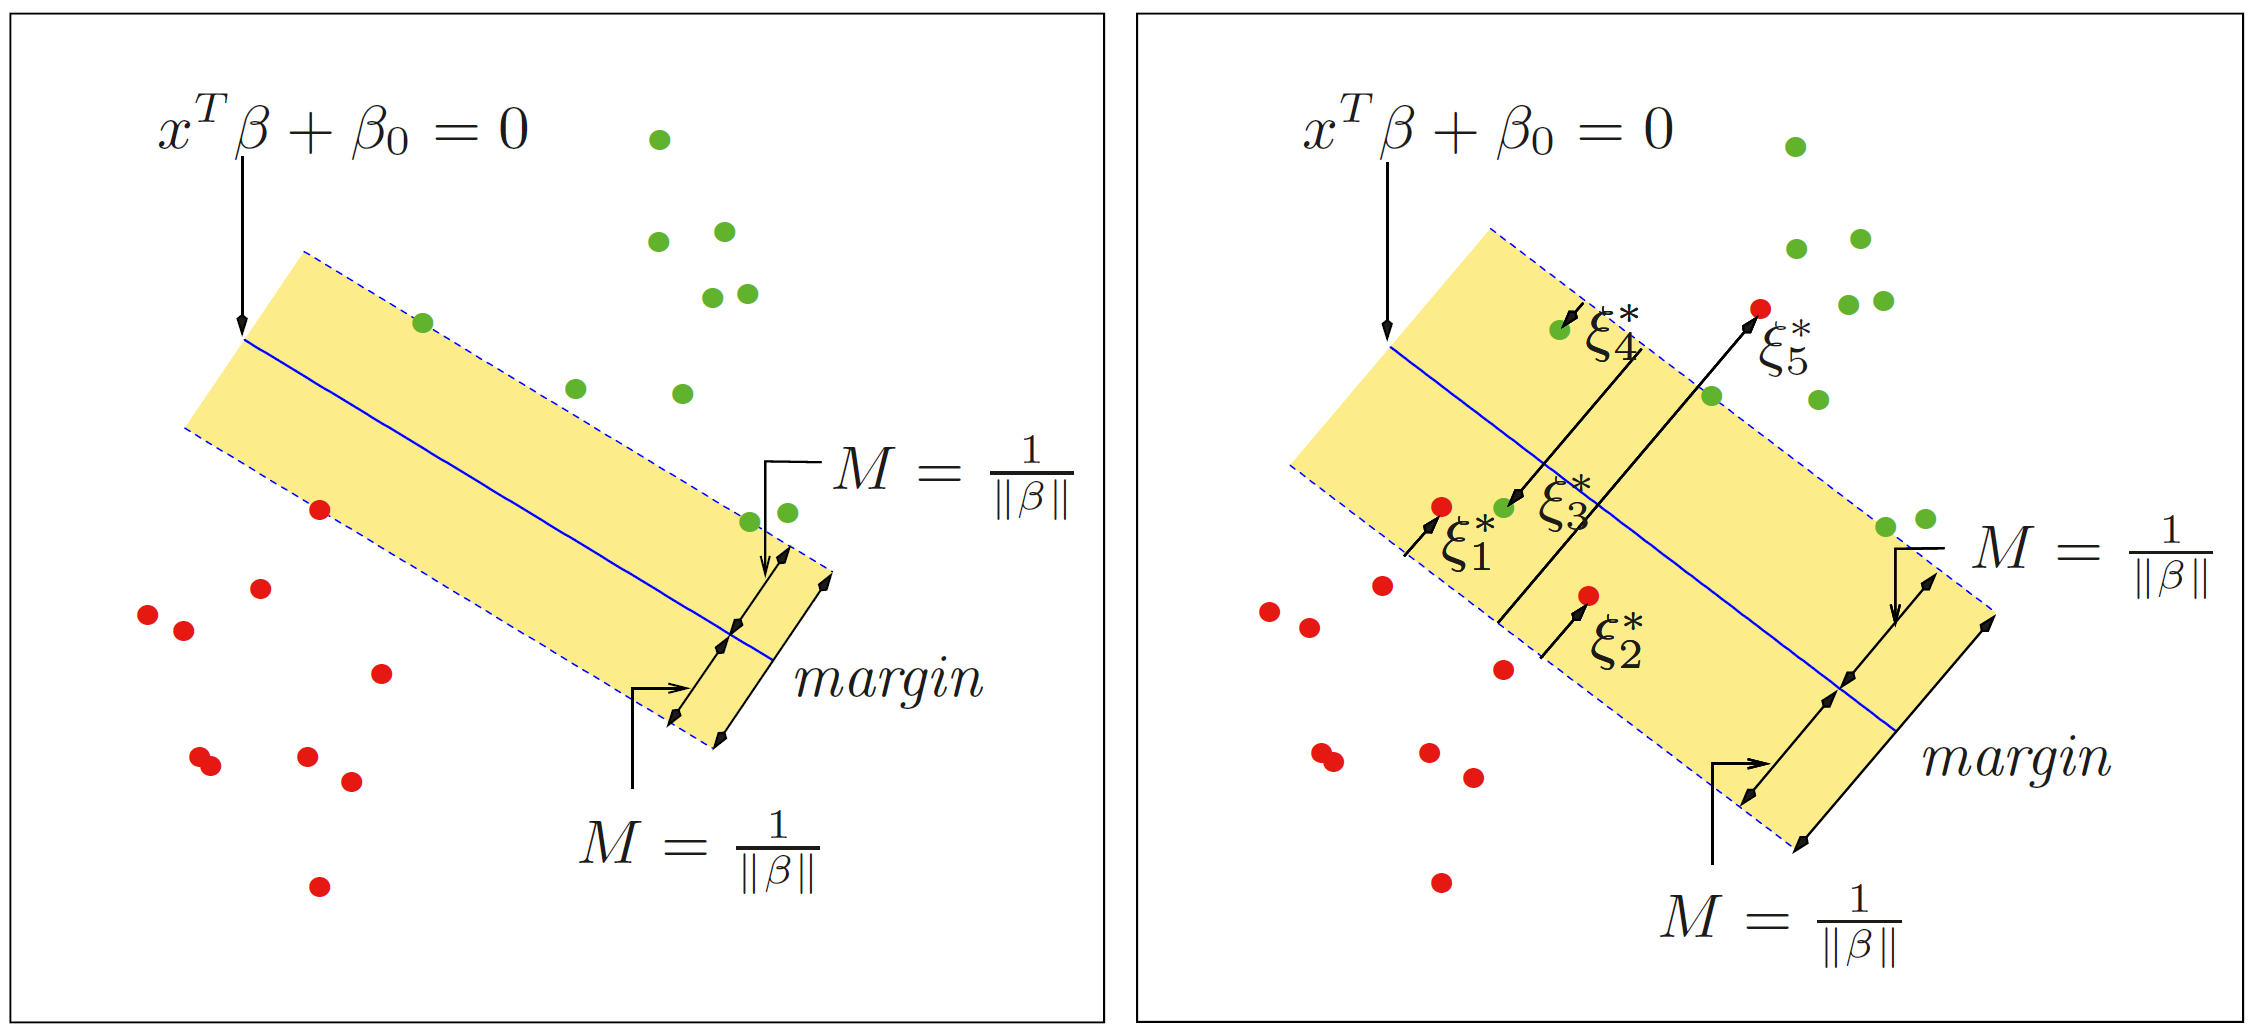
\includegraphics[width=0.55\textwidth]{../imgs/svm_hastie_2009.png}
        \caption{SVM. Left: A separable case; Right: A non-separable case. The 
        vectors $\xi_j^*$ are the support vectors \footcite{hastie2009elements}.}
    \end{figure}
    % ksi
\end{frame}

%-------------------------------------------------------------------------------
\begin{frame}[t]
    \frametitle{Support Vector Machine (SVM)}
    Explain briefly how an SVM is trained.

    \begin{itemize}
        \item A technique for constructing an optimal separating hyperplane between two classes
        \item The margin $M$ is $\frac{1}{\|\beta\|}$; Minimize $\|\beta\|$ (Maximize margin)
        \item \textbf{Hard-margin:} the training data is linearly separable
        \item \textbf{Soft-margin:} the data are not linearly separable, minimize the observations on the wrong side by minimizing the hinge loss using Lagrangian multiplier.
        \item \textbf{Kernel function} is used for the non-linear boundaries. e.g.: 2-degree polynomial $\phi(x)=x^2$ 
    \end{itemize}

\end{frame}

%-------------------------------------------------------------------------------
\begin{frame}[t]
    \frametitle{Multi-class Classification}
    What strategies are SVM use when the data have more than two classes?
    \pause

    \begin{itemize}
        \item \textbf{One-Vs-Rest (OVR):} Example: Three output classes: A, B, C. 
        Solve 3 binary classified problem: 
            \begin{enumerate}
                \item A vs. (B, C)
                \item B vs. (A, C)
                \item C vs. (A, B)
            \end{enumerate}
        \item \textbf{One-Vs-One (OVO):} Train N choose 2 classifiers, ${N \choose 2} = \frac{N \cdot (N-1)}{2}$
            \begin{enumerate}
                \item A vs. B
                \item A vs. C
                \item B vs. C
            \end{enumerate}
    \end{itemize}

\end{frame}

%-------------------------------------------------------------------------------
\begin{frame}[t]
    \frametitle{Support Vector Machine}
    What the difference between SVM and logistic regression?
    \pause

    \begin{itemize}
        \item SVM maximizes the margin between the closest support vectors
        \item Logistic regression maximize the posterior class probability (Different loss function)
        \item SVM is deterministic and LR is probabilistic
        \item SVM can be used for both classification and regression
    \end{itemize}

    \begin{figure}
        \centering
        \small
        \begin{subfigure}[t]{0.25\linewidth}
            \captionsetup{justification=centering}
            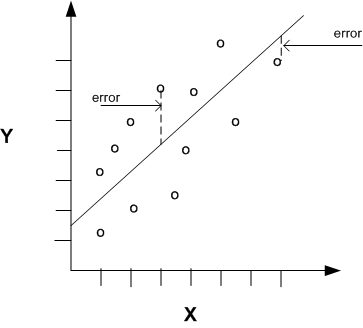
\includegraphics[width=\linewidth]{../imgs/Linear-regression.png}
            \caption{Linear Regression}
        \end{subfigure}
        \begin{subfigure}[t]{0.30\linewidth}
            \captionsetup{justification=centering}
            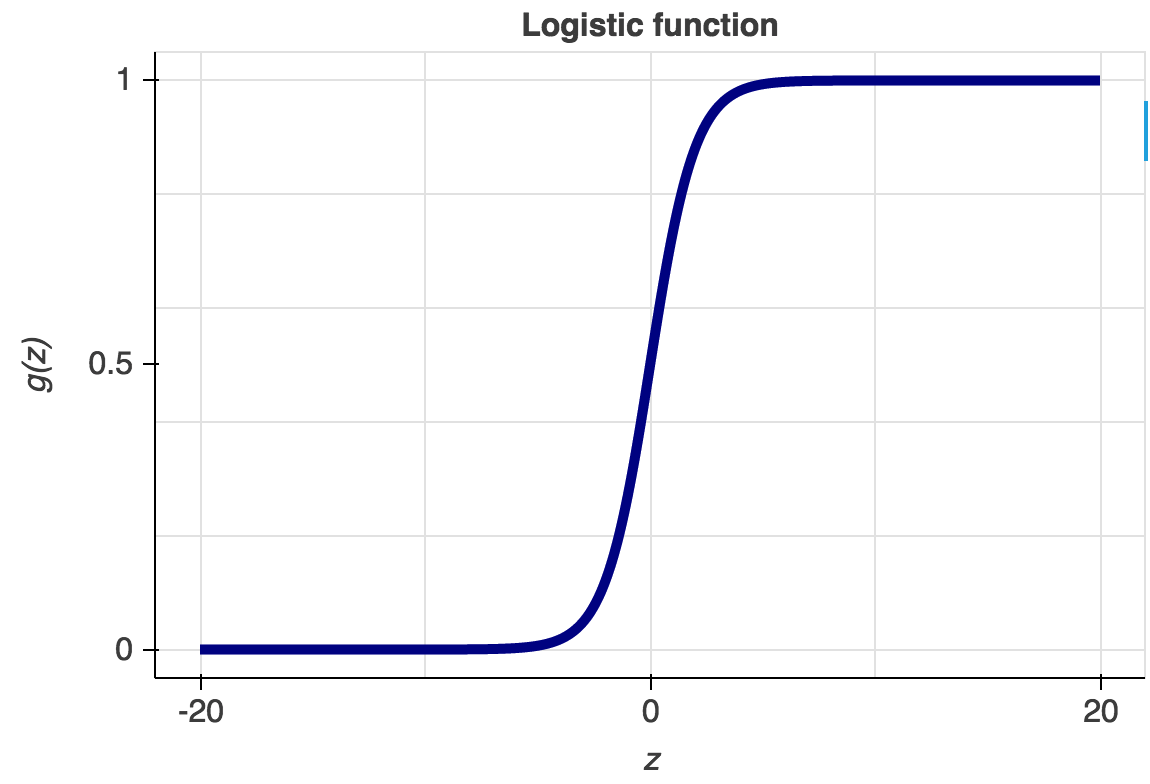
\includegraphics[width=\linewidth]{../imgs/lr.png}
            \caption{Logistic Regression}
        \end{subfigure}
        \begin{subfigure}[t]{0.30\linewidth}
            \captionsetup{justification=centering}
            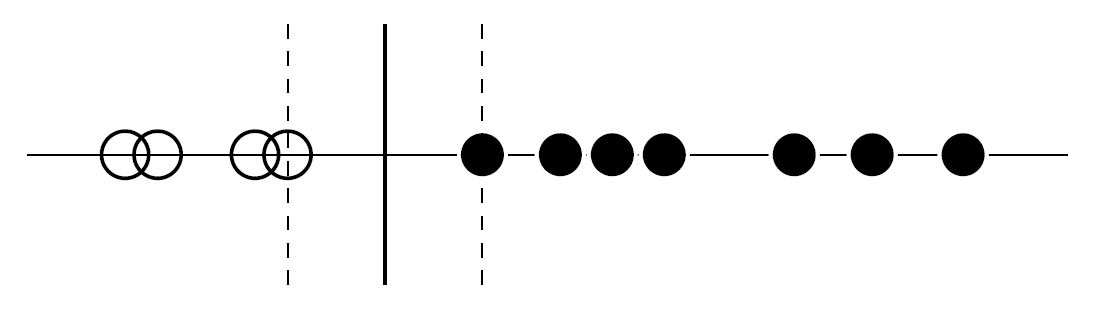
\includegraphics[width=\linewidth]{../imgs/svm.png}
            \caption{SVM}
        \end{subfigure}
    \end{figure}

\end{frame}

%-------------------------------------------------------------------------------
\begin{frame}[t]
    \frametitle{Support Vector Machine}
    How do SVMs compare to simple instance-based learning approaches such as k-Nearest Neighbour?
    \pause

    \begin{itemize}
        \item Both can be thought of as instance based learners
        \item SVM doesn’t need to store all training samples
        \item SVM outperforms kNN in high dimensional data
    \end{itemize}

\end{frame}

%-------------------------------------------------------------------------------
\begin{frame}[t]
    \frametitle{Parameters in SVM}
    Which hyper-parameters should you tune?
    \pause

    \begin{itemize}
        \item SVM is NOT scale invariant. Before training, normalize your data.
        \item \textbf{Complexity parameter:} The penalty parameter $c$ of the error term. 
        In \textit{sklearn}, the default value is 1. If the data is noisy, decrease it (Less penalty for misclassification.). 
        If the data is highly non-linear, increase it. $c$ can take value larger than 1, e.g.: $c \in [0.1, 100]$
        \item \textbf{kernel}: Linear, polynomial, sigmoid, Radial Basis Function (RBF)
        \item For non-linear kernels, $\gamma$ is the kernel coefficient. The default value is $\frac{1}{\text{n\_features}}$.
        If $\gamma$ is small, the model prefers linear-like decision boundary. Large value may lead to overfitting.
    \end{itemize}

\end{frame}

%-------------------------------------------------------------------------------
% \section{Markov Decision Process (MDP)}
% \begin{frame}[t]
% \frametitle{Markov Decision Process (MDP)}


% \end{frame}

% %-------------------------------------------------------------------------------
% \section{Q-Learning}
% \begin{frame}[t]
% \frametitle{Q-Learning}

% \end{frame}

\end{document}


